\documentclass[a4j,8pt,twocolumn]{extarticle}

% ---------------

\usepackage{winf-paper}
\usepackage{amsmath,amssymb,ascmac}
\usepackage{latexsym}
\usepackage{ulem}
\usepackage{subfig}
\usepackage{xcolor}
\usepackage[dvipdfmx]{graphicx}
\usepackage{url}

\captionsetup[subfigure]{labelformat=simple}
\renewcommand{\thesubfigure}{(\alph{subfigure})}

\title{距離学習を導入したCenterNetによる腹部超音波画像からの肝腫瘍検出と分類}
\author{原 英吾$^\dagger$ \qquad 道満 恵介$^\dagger$ \qquad 目加田 慶人$^\dagger$ \qquad 西田 直生志$^\ddagger$ \qquad 工藤 正俊$^\ddagger$}
\affiliation{%
    $^\dagger$中京大学 工学部 \\ Email: \url{hara.e@md.sist.chukyo-u.ac.jp}, \url{{kdoman,y-mekada}@sist.chukyo-u.ac.jp}\\
    \vspace{1ex}
    $^\ddagger$近畿大学 医学部 \\ Email: \url{{naoshi, m-kudo}@med.kindai.ac.jp}
}

\begin{document}
    \maketitle
    \thispagestyle{empty}

    \section{はじめに}
        2020年には,世界中で83万人以上の方が肝臓がんで死亡しており,世界のがん死亡原因の第3位である.
        また,近年,超音波検査は肝がんの初期診断に有効な方法と考えられている.
        しかし,器具の操作と診断を同時に行わなければならないことから腹部超音波検査は難易度が高いとされている.
        そのため,腹部腫瘍の検出や分類などはコンピュータを用いた診断が求められている.

        従来は,図\ref{fig:us}の様な与えられた超音波画像に対して腫瘍の検出後に,切り出された腫瘍領域\cite{yamagishi2022detection}を分類する\cite{nishida2022artificial}という2段階の推論ステップによって構成されている.

        山岸らの先行研究\cite{yamagishi2022detection}により,YOLOv5による腫瘍検出手法が提案されている.
        YOLOv5とは,Ultralytics社により開発されており,2020年6月に公開された画像中の物体認識ライブラリである.
        この先行研究では,IoUしきい値が0.25で信頼度のしきい値を0.3とした時に,再現率,適合率,F1スコアがそれぞれ0.855,0.896,0.875となることが報告されている.
        しかし,YOLO系統のモデルは様々なアスペクト比の物体を検出するという前提のため,本稿の問題設定に適していない可能性が高い.

        西田らの先行研究\cite{nishida2022artificial}により,図~\ref{fig:cyst},\ref{fig:hemangioma},\ref{fig:hcc},\ref{fig:meta}の様な切り取られた腫瘍画像に対して,VGG16\cite{simonyan2021very}ベースのCNNモデルによる腫瘍分類手法が提案されており,accuracyが0.8909であることが報告されている.
        ここで,検出段階において画像を切り取らないことで,分類時に大域特徴を使用できるため精度の向上が見込めると考える.

        本稿では,図~\ref{fig:ex}に示すように,単純嚢胞(図~\ref{fig:cyst}),血管腫(図~\ref{fig:hemangioma}),肝細胞がん(図~\ref{fig:hcc}),そして転移性肝がん(図~\ref{fig:meta})の検出と分類を同時に行う.
        なお,後者2症状は悪性であるため極力未検出を抑制する必要がある.

        \begin{figure}[t]
            \centering
            \subfloat[実際の診断で使われる画像]{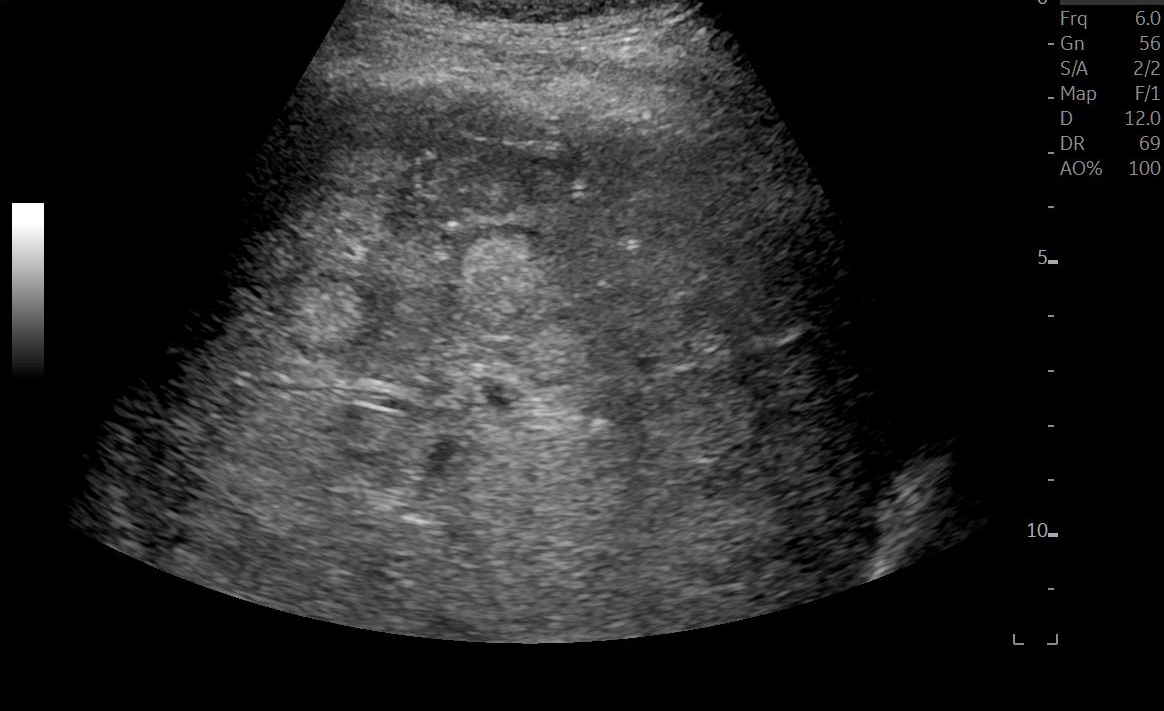
\includegraphics[width=.98\linewidth]{../fig/us.png} \label{fig:us}}

            \subfloat[単純嚢胞]{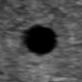
\includegraphics[width=.235\linewidth]{../fig/cyst.png} \label{fig:cyst}}
            \hfill
            \subfloat[血管腫]{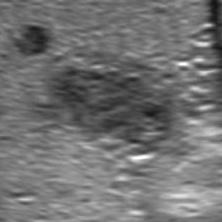
\includegraphics[width=.235\linewidth]{../fig/hemangioma.png} \label{fig:hemangioma}}
            \hfill
            \subfloat[肝細胞がん]{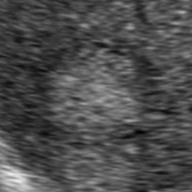
\includegraphics[width=.235\linewidth]{../fig/hcc.png} \label{fig:hcc}}
            \hfill
            \subfloat[転移性肝がん]{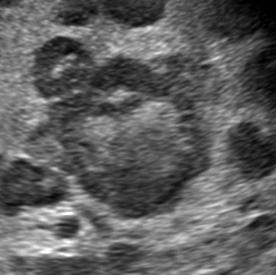
\includegraphics[width=.235\linewidth]{../fig/meta.png} \label{fig:meta}}
            \caption{実験で用いる超音波画像例}
            \label{fig:ex}
        \end{figure}

    \section{提案手法}
        \label{sec:propose}
        本稿では,切り取られた腫瘍画像を入力としてSimSiam\cite{chen2021exploring}で距離学習をさせたバックボーンネットワークを用いてCenterNet\cite{zhou2019objects}をファインチューニングし,1段階の推論手法を提案する.
        図\ref{fig:architecture}に示すように,腹部超音波画像に影像される肝腫瘍は形状が円形であることから,CenterNetのみを用いて推論することで効果的に腫瘍の検出・分類できると考える.

        CenterNetに用いるバックボーンネットワークは,切り取られた腫瘍の画像を入力としてSimSiamを用いた距離学習を行う.その後,\ref{fig:us}の様に全体が映っている画像を用いてファインチューニングする.
        SimSiamは単純な構造を持ち,少ないバッチサイズでも検出と分類の両タスクに有効な特徴を学習することが可能な上,図\ref{fig:ex}に示す様に4種類の腫瘍が画像の見た目が大きく異なっていることから採用した.

        また,従来手法よりも推論に使用するモデルを減らすことで,メモリの削減や推論速度の上昇が見込める上に,超音波画像全体を用いて腫瘍の分類も行うため4クラス検出の高精度化が見込める.

        このような枠組みにより,本手法は入力画像から肝腫瘍の位置や大きさ,種類(keypoint heatmap)を出力している.

        \begin{figure*}[!ht]
            \centering
            \hspace{3em}
            \subfloat[事前に距離学習で使用するSimSiamモデル]{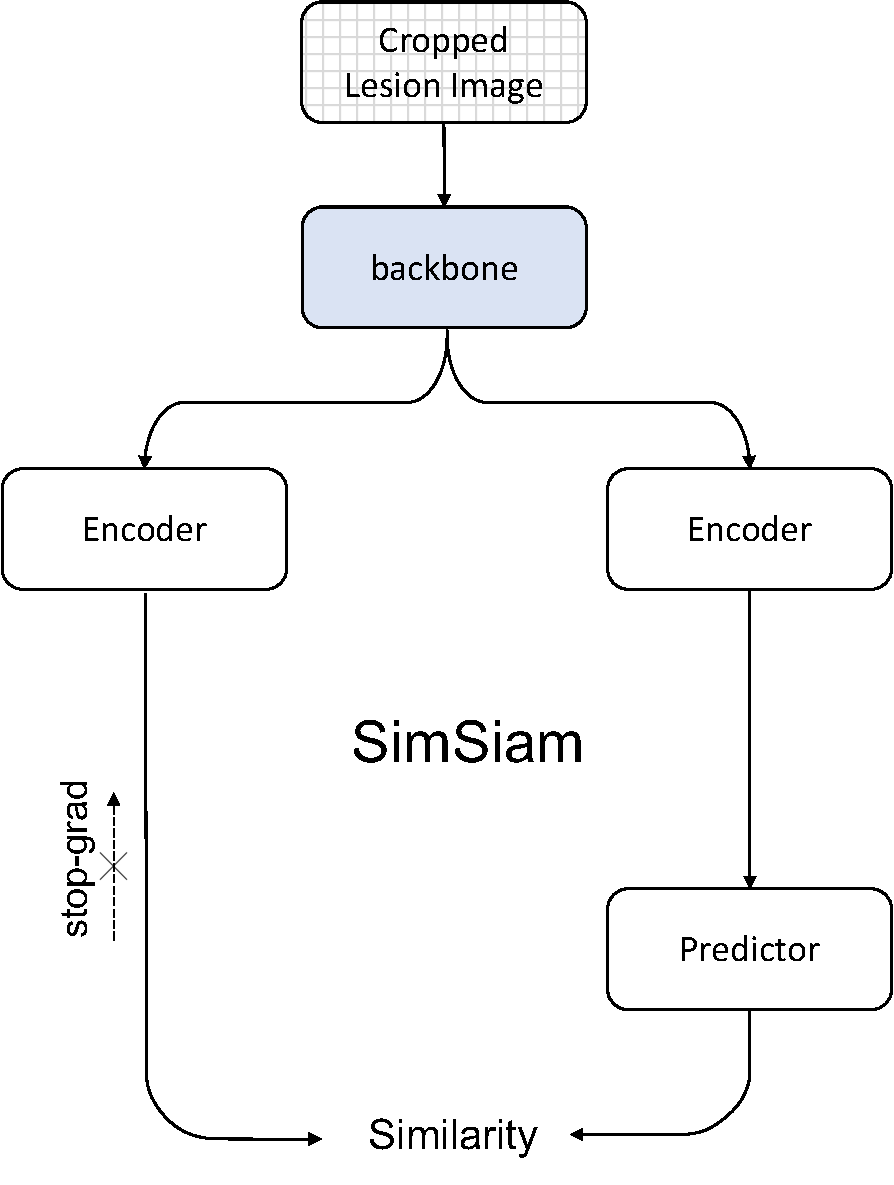
\includegraphics[height=58ex]{../fig/simsiam.pdf} \label{fig:simsiam}}
            \hfill
            \subfloat[学習及び推論で用いるCenterNetのモデル]{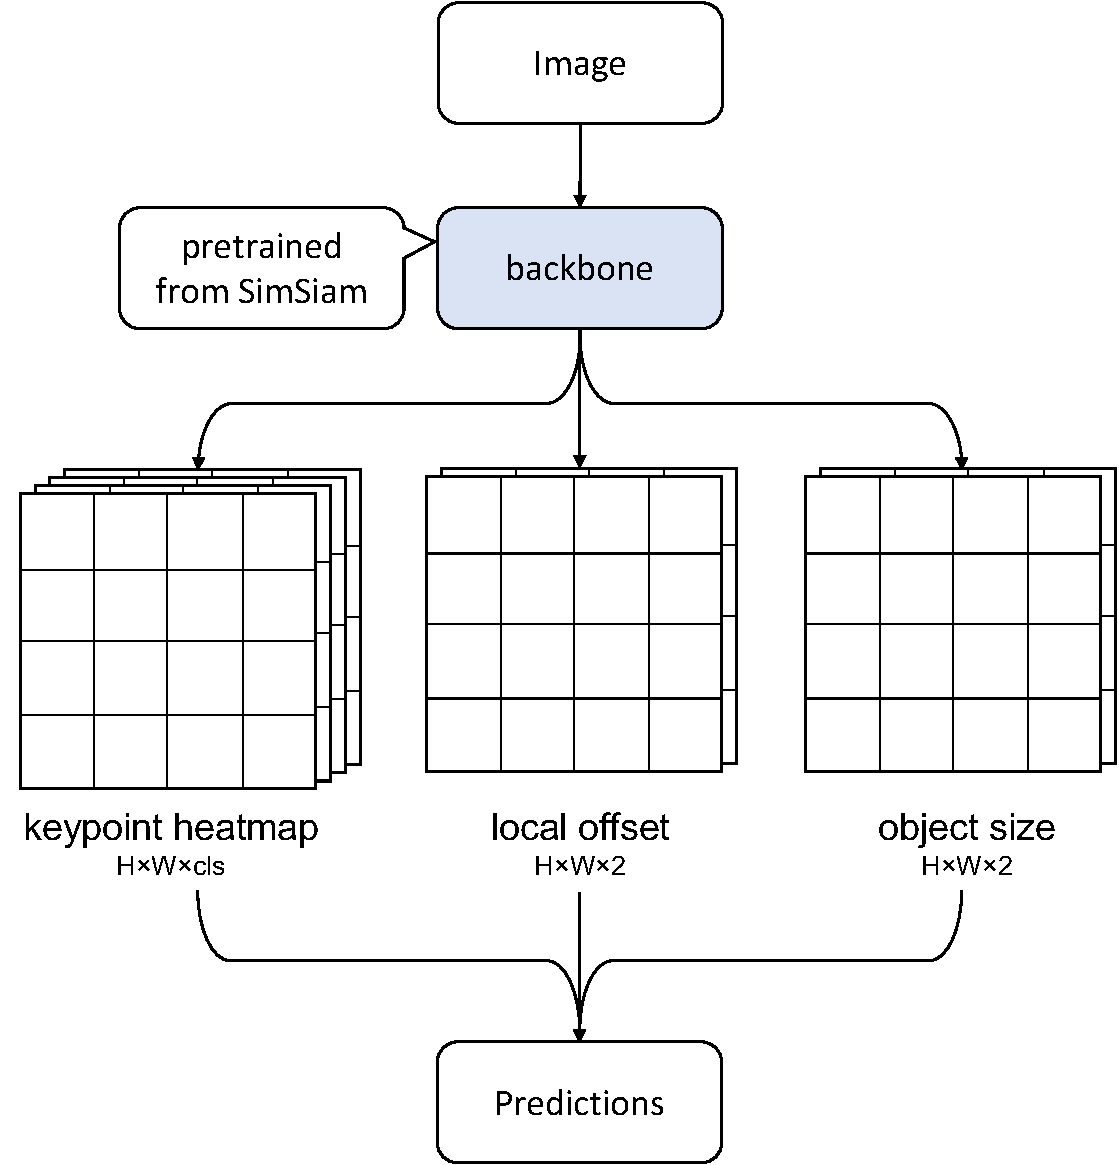
\includegraphics[height=58ex]{../fig/centernet.pdf} \label{fig:centernet}}
            \hspace{3em}
            \caption{提案手法の構造: バックボーンネットワークの事前学習に用いるSimSiamと推論を行うCenterNet}
            \label{fig:architecture}
        \end{figure*}

    \section{実験}
        本節では,\ref{sec:dataset}節で作成したデータセットを用いて,\ref{sec:train}節の学習を行う.そして,最後の\ref{sec:eval}節で提案手法の有効性を確かめる評価実験を行った.

        \subsection{データセット}
        \label{sec:dataset}
            本実験では超音波医学会(AMED)から提供されている全89,903枚の腹部超音波画像を,表\ref{tab:dataset}で示す様にtrain : test : validation$ = 8 : 1 : 1$と分割してモデルを学習させ,評価を行った.

            \begin{table}[t]
                \centering
                \caption{データセット分割後のそれぞれの枚数}
                \label{tab:dataset}
                    \begin{tabular}{l|rcr|c} \hline
                        \multicolumn{1}{c|}{診断名} & \multicolumn{1}{c}{train} & validation & \multicolumn{1}{c|}{test} & 合計 \\ \hline
                        単純嚢胞 & 24,217 & 3,018 & 3,037 & 30,272 \\
                        血管腫 & 23,749 & 3,059 & 2,962 & 29,770 \\
                        肝細胞がん & 10,934 & 1,310 & 1,371 & 13,615 \\
                        転移性肝がん & 8,222 & 1,003 & 1,021 & 10,246 \\ \hline
                        合計 & 67,122 & 8,390 & 8,391 & 83,903 \\ \hline
                    \end{tabular}
            \end{table}

        \subsection{データセットの問題}
            \label{sec:data_prob}
            このデータセットの特性として,以下の3点が挙げられる.
            \begin{enumerate}
                \item 画像内にカラーのスケールが映り込んでいる場合がある \label{scale}
                \item ほぼ同じ画像が混ざっている \label{same}
                \item 複数の腫瘍が写っていてもアノテーションが1つしかない \label{anno}
            \end{enumerate}
            (\ref{scale}), (\ref{same})については頑健性低下の大きな要因になるため,それぞれ中島ら\cite{nakashima2020study}と同様の手法でデータセットを作成した.具体的には,スケールを乱数で消すことやHash値による類似画像の削除により,データクレンジングを行っている.
            また,(\ref{anno})に関しては,図~\ref{fig:meta}に示す様に,転移性肝がんの他部位にも同様に転移しやすいという性質により,主に転移性肝がんの検出精度を下げる大きな原因になることがわかっている.

        \subsection{提案モデルの学習}
            \label{sec:train}
            \ref{sec:propose}節で提案したSimSiamとCenterNetを\ref{sec:dataset}節で作成した学習データで学習させた.
            その際に,表\ref{tab:param}に示すハイパーパラメータを用いた.なお,CenterNetの誤差関数に関しては,keypoint heatmapでGaussian Focal Lossを,local offsetとobject sizeでL1損失を用いているため複数記述している.

            また,SimSiamで学習させた初期重みを有効活用させるために,CenterNetの学習ではバックボーンネットワークの重みを固定し,学習を進めるにつれて段階的に解除した.

            \begin{table}[!t]
                \centering
                \caption{学習で使用するモデルとそのハイパーパラメータ}
                \label{tab:param}
                    \begin{tabular}{l|cc} \hline
                        & SimSiam & CenterNet \\ \hline
                        バッチサイズ &  64 &  16 \\
                        エポック &  300 &  300 \\
                        学習率 & $1.0 \times 10^{-4}$ & $5.0 \times 10^{-5}$ \\
                        入力サイズ & $512 \times 512$ & $512 \times 512$ \\
                        最適化関数 & SGD & SGD \\
                        誤差関数 & Cosine Similarity & L1 Gaussian Focal \\ \hline
                    \end{tabular}
            \end{table}

            \subsection{評価実験}
                \label{sec:eval}
                学習が終了したモデルについては,表\ref{tab:dataset}に示されたテストデータを用いて4クラス検出の評価実験を行った.
                その際,先行研究に則り,IoUのしきい値は0.25,信頼度のしきい値は0.00から1.00まで0.05ずつ変化させて計測したF1値が最大となる時の値とする.
                今回の評価実験では,信頼度のしきい値は0.40となった.

    \section{結果}
        \label{sec:result}
        \ref{sec:eval}節の条件のもとでの検出結果(図\ref{fig:detection}),提案手法の混同行列(図\ref{fig:cmat}),そしてその集計データ(表\ref{tab:metric})を示す.
        なお,図~\ref{fig:detection}と図~\ref{fig:cmat}に関しては,単純嚢胞(Cyst),肝細胞がん(HCC),血管腫(Hem.),転移性肝がん(Meta)としている.
        また,比較手法としてYOLOX\cite{ge2021yolox}で4クラス分類を行った結果を図\ref{fig:cmat_yolox},表\ref{tab:metric_yolox}に示す.
        そして,表\ref{tab:comparison}に,手法毎における使用メモリ,推論速度,そして4クラス検出精度の比較結果を示す.

        \begin{table}[t]
            \centering
            \caption{提案手法を用いたモデルでの評価指標毎の値}
            \label{tab:metric}
                \begin{tabular}{l|rrr|ccc} \hline
                    診断名 & \multicolumn{1}{c}{腫瘍数} & \multicolumn{1}{c}{FP} & \multicolumn{1}{c|}{FN} & 適合率 & 再現率 & F1 \\ \hline
                    Cyst & 3,037 & 492 & 357 & 0.832 & 0.873 & 0.852 \\
                    HCC & 1,371 & 168 & 339 & 0.722 & 0.601 & 0.657 \\
                    Hem. & 398 & 301 & 465 & 0.828 & 0.796 & 0.812 \\
                    Meta & 1,021 & 172 & 290 & 0.619 & 0.543 & 0.578 \\ \hline
                    合計 & 8,391 & 1,133 & 1,451 & 0.750 & 0.703 & 0.725 \\ \hline
                \end{tabular}
        \end{table}

        \begin{table}[t]
            \centering
            \caption{YOLOXでの評価指標毎の値}
            \label{tab:metric_yolox}
            \begin{tabular}{l|rrr|ccc} \hline
                診断名 & \multicolumn{1}{c}{腫瘍数} & \multicolumn{1}{c}{FP} & \multicolumn{1}{c|}{FN} & 適合率 & 再現率 & F1 \\ \hline
                Cyst & 3,037 & 851 & 297 & 0.741 & 0.892 & 0.809 \\
                HCC & 1,371 & 371 & 371 & 0.471 & 0.591 & 0.524 \\
                Hem. & 2,962 & 468 & 591 & 0.740 & 0.744 & 0.742 \\
                Meta & 1,021 & 28 & 339 & 0.686 & 0.106 & 0.183 \\ \hline
                合計 & 8,391 & 1,718 & 1,598 & 0.685 & 0.695 & 0.690 \\ \hline
            \end{tabular}
        \end{table}

        \begin{table*}[!t]
            \centering
            \caption{従来手法,YOLOXと提案手法の比較}
            \label{tab:comparison}
            \resizebox{\width}{!}{
                \begin{tabular}{l|rr|rrr|r} \hline
                    & 使用メモリ(MB) & 推論速度(/sec)& 再現率$_{det}$ & 精度$_{cls}$ & \multicolumn{1}{c|}{4クラス検出精度} & \multicolumn{1}{c}{信頼度} \\ \hline
                    \multicolumn{1}{c|}{従来手法\cite{yamagishi2022detection,nishida2022artificial}} & 3898.3 & 0.0272 & 0.8550 & 0.8909 & 0.7617 $(\approx 0.8550 \times 0.8909)$ & 0.30 \\
                    YOLOX\cite{ge2021yolox} & 4178.9 & 0.0167 & 0.8096 & 0.8447 & 0.6839 $(\approx 0.8096 \times 0.8447)$ & 0.35 \\
                    \textbf{提案手法} & \textbf{1838.2} & \textbf{0.0095} & \textbf{0.8271} & \textbf{0.9206} & \textbf{0.7614} $(\approx 0.8271 \times 0.9206)$ & \textbf{0.40} \\ \hline
                \end{tabular}
            }
        \end{table*}

        これらの結果から,未検出,過検出,適合率,再現率,使用メモリ,そして推論速度の全ての評価項目において提案手法がYOLOXを上回っている.

        \begin{figure}[!t]
            \centering
            \subfloat[単純嚢胞の検出例]{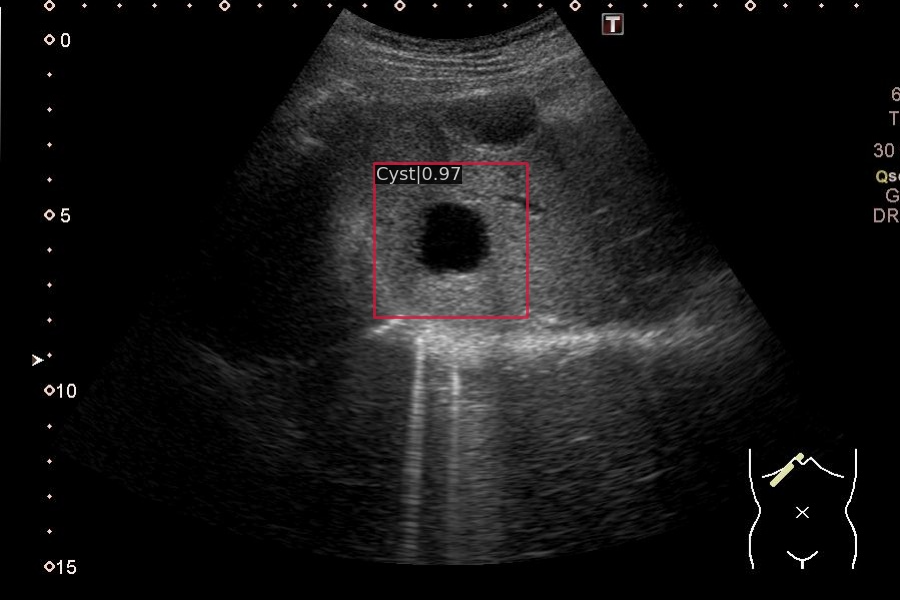
\includegraphics[width=.48\linewidth]{../fig/center_cyst.png} \label{fig:center_cyst}}
            \subfloat[血管腫の検出例(嚢胞と血管の誤り)]{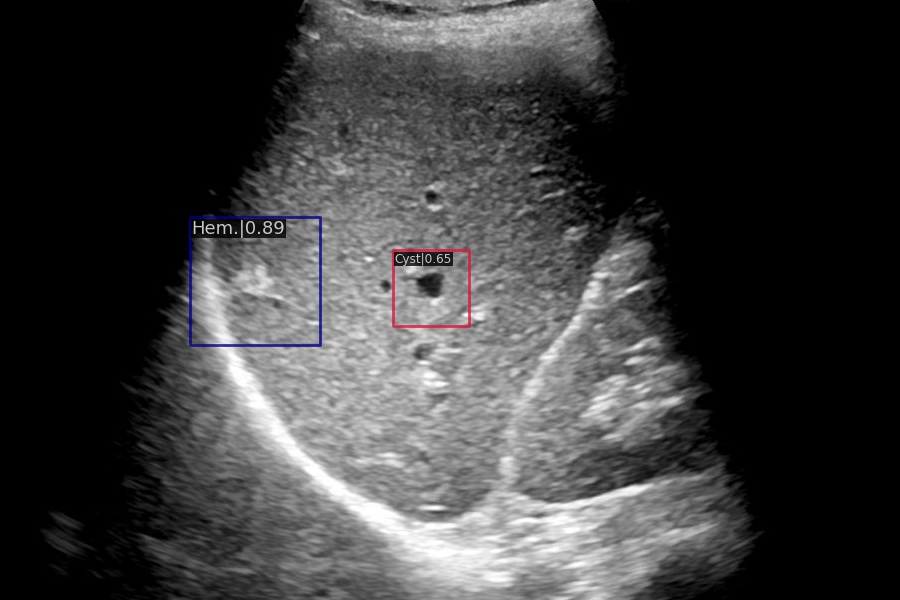
\includegraphics[width=.48\linewidth]{../fig/center_hem.png} \label{fig:center_hem}}

            \subfloat[肝細胞がんの検出例]{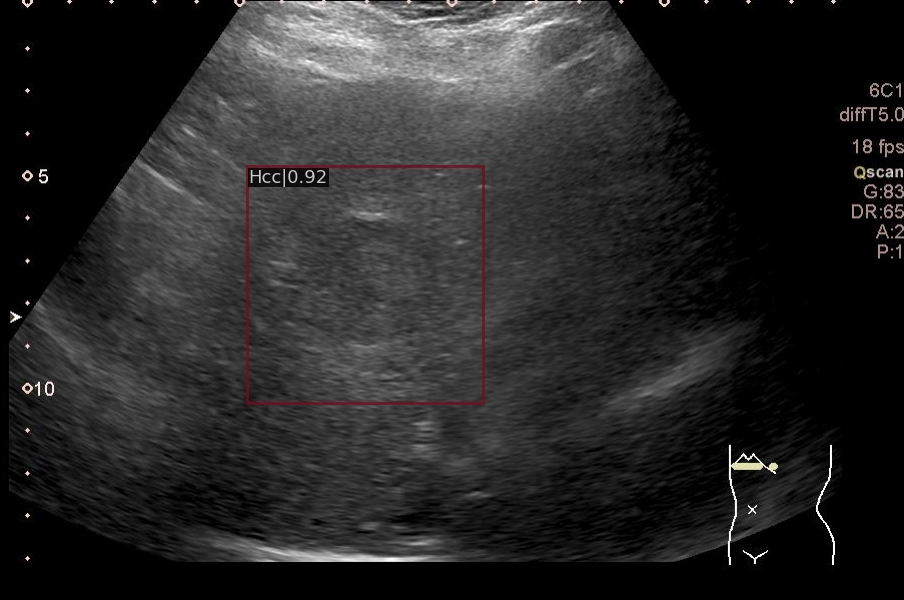
\includegraphics[width=.48\linewidth]{../fig/center_hcc.png} \label{fig:center_hcc}}
            \subfloat[転移性肝がん(複数)の検出例]{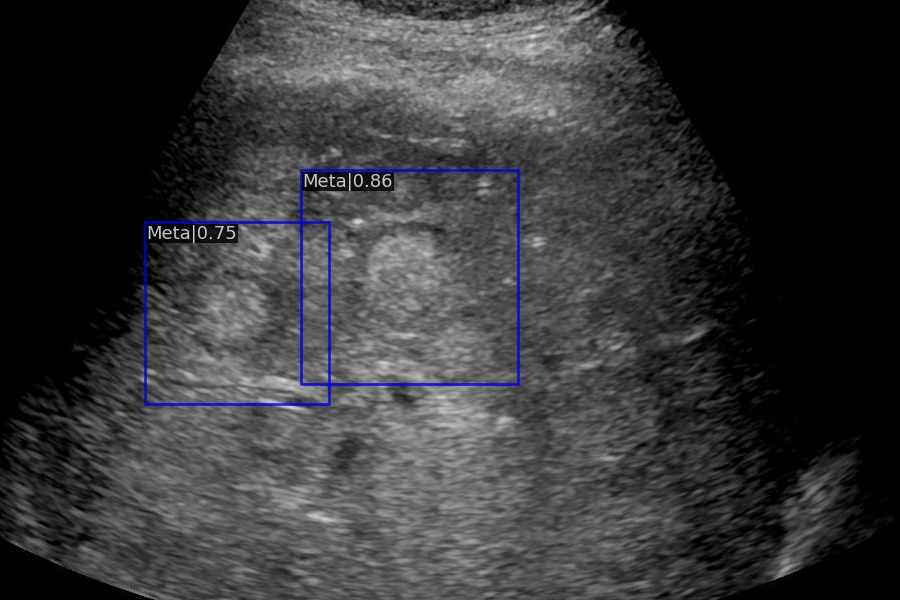
\includegraphics[width=.48\linewidth]{../fig/center_meta.png} \label{fig:center_meta}}
            \caption{提案手法での4クラス検出例}
            \label{fig:detection}
        \end{figure}

        \begin{figure}[!t]
            \centering
            \subfloat[提案手法での混同行列]{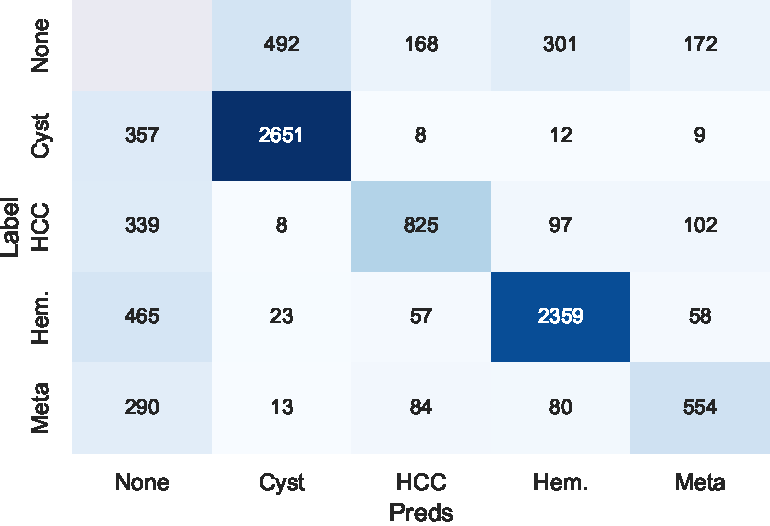
\includegraphics[width=.98\linewidth]{../fig/heatmap_centernet_stepwise2.pdf} \label{fig:cmat_centernet}}

            \subfloat[YOLOXでの混同行列]{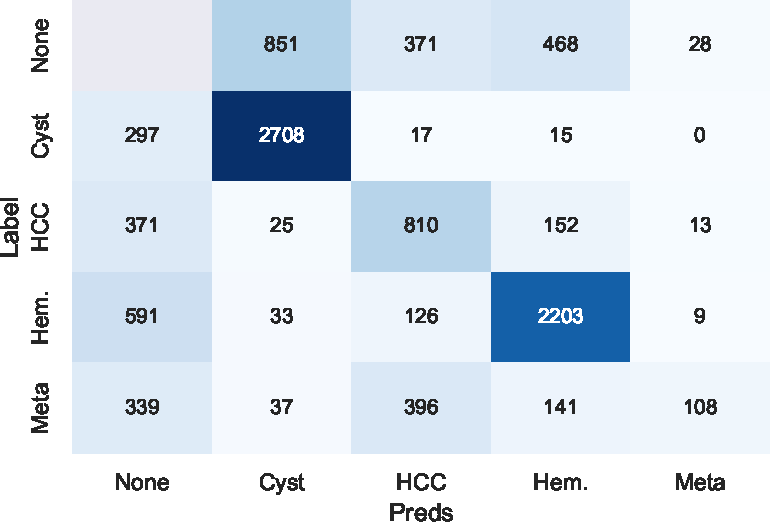
\includegraphics[width=.98\linewidth]{../fig/heatmap_yolox.pdf} \label{fig:cmat_yolox}}
            \caption{提案手法とYOLOXで4クラス分類を行った際の比較}
            \label{fig:cmat}
        \end{figure}

    \section{考察}
        \label{sec:consideration}
        \ref{sec:result}節から,提案手法の再現率とAccuracyを算出し,4クラス検出結果の比較を行った結果を表\ref{tab:comparison}に示す.
        4クラス分類精度が向上している要因として,SimSiamによる距離学習や,従来手法で得ることのできなかった画像の大域特徴を有効活用できたことが挙げられる.
        一方で,検出精度が低下しているのはSimSiamによるバックボーンネットワークに対する4クラスの距離学習で検出に不向きな特徴量を学習してしまったのではないかと考えられる.
        また,提案手法は従来手法よりも省メモリかつ高速に推論を行うことができることが示された.
        これにより,エッジデバイスでの実装が容易になったと考えられる.
        従って,提案手法による一定の有効性を確認することができた.

        表\ref{tab:metric}に関して,悪性腫瘍(肝細胞がん,転移性肝がん)の再現率が良性腫瘍(単純嚢胞,血管腫)に比べて低く,診断が難しいと言える.
        これは,データセットに含まれる悪性腫瘍の数が少ない(表~\ref{tab:dataset})ことによる学習データ不足が大きな原因だと考えられる.
        特に転移性肝がんの精度が低い問題に関しては,データの偏りに加えてアノテーション不足(\ref{sec:data_prob}節)に依る所も大きいと推測する.

        図\ref{fig:detection}の様に,高精度で4クラスの検出と分類ができていることが定性的にわかる.しかし,血管を単純嚢胞(Cyst)と誤検出(図~\ref{fig:center_hem})してしまったり,未検出の腫瘍が複数存在する(図\ref{fig:center_meta})している.
        これらはそれぞれ,図\ref{fig:cyst}に示す様に症状の特性が血管と似ていることや,\ref{sec:dataset}節で述べたアノテーションの問題が大きな要因であると考えられる.解決にはモデルの改善もそうだが,実際の診断で用いるような超音波動画等の入力による腫瘍の追跡処理が必要であると考える.

    \section{まとめ}
        腹部超音波画像から肝腫瘍を同時に検出・分類する方法として,SimSiamに基づく距離学習を用いたCenterNetによる1段階手法を提案した.
        この提案手法は,従来の検出された腫瘍領域に対して4クラスの分類を行う,2段階手法と同等の高い分類精度を達成できることを確認した.また,この提案手法は従来手法よりも省メモリかつ高速に推論が可能である.

        しかし,分類精度は向上したが検出精度が低下してしまったことから,腫瘍の検出と腫瘍の分類に必要な特徴量が異なっていると考えられる.
        したがって今後は,検出と分類の両方に適したモデルとなるような改良をしていく予定であり,例えば,検出headと分類headをバックボーンネットワークから分離するなどの研究を行うことを想定している.

    \section*{謝辞}
        本研究の一部は,AMED革新的がん医療実用化研究事業および日本学術振興会科研費の援助による.

    \bibliographystyle{spiebib}
    \bibliography{paperlist}
\end{document}
